% !TEX TS-program = pdflatex
% !TEX encoding = UTF-8 Unicode
% !TEX root = ../main.tex
% !TEX spellcheck = en-US
% ****************************************************************************************
% File: discussion.tex
% Author: Jakob Spindler
% Date: 2024-10-16
% ****************************************************************************************
\chapter{Discussion}
\label{chapter:discussion}

The Results show that the use of an X-cap alone is sufficient enough to reduce the conducted emissions of the buck converter to a level that is compliant with the EN 55022/32 standard. This implementation is also the most cost-effective and simplest to implement, however, it creates a high output voltage ripple/spiking that spans aproxiamtely \qty{1}{\volt} as can be seen in \autoref{fig:x_cap_ripple}. This ripple is not ideal for sensitive applications and may require further filtering.

The use of a \gls{acr:cmc} in addition to the X-cap further reduces the overall emissions, but the difference is marginal. Additionally, a substantial spike in \gls{acr:cm} emissions is observed at \qty{1}{\mega\hertz} as can be seen in \autoref{fig:cmc_x_cap_emc}. This spike is likely due to the resonance of the \gls{acr:cmc} and the parasitic capacitance of the buck converter and leads to a no-pass criterion for the EN 55022/32 standard.

The use of Y-caps in addition to the X-cap and the \gls{acr:cmc} reduces the conducted \gls{acr:cm} emissions of the buck converter which are now well below the limit of the EN 55022/32 standard. The output voltage ripple is also reduced to a level that is acceptable for sensitive applications as can be seen in \autoref{fig:cmc_x_cap_y_cap_vout}.

In conclusion, the use of an X-cap alone is sufficient to reduce the conducted emissions of the buck converter to an acceptable level. 
By implementing a \gls{acr:cmc} and Y-caps in addition to the X-cap, the emissions can be further reduced whilst also reducing the output voltage ripple.

\section{PCB Layout Considerations}
\label{section:pcb_layout_considerations}
For our implemented methods to be efficte in a real world scenario, a fitting \Gls{acr:pcb} layout is crucial. The following points should be considered \autocite{LT8618DatasheetProduct}:
\begin{itemize}
    \item Place the input capacitor ($C_{IN}$) adjacent to the VIN and GND pins to minimize the loop formed by the input capacitor.
    \item If using a large input capacitor, place a small case/value capacitor close to the VIN and GND pins and the larger capacitor further away.
    \item Place the inductor and output capacitor (COUT) on the same side of the circuit board as the input capacitor.
    \item Ensure connections for the input capacitor, inductor, and output capacitor are made on the same layer.
    \item Place a local, unbroken ground plane under the application circuit on the layer closest to the surface layer.
    \item Keep the SW and BOOST nodes as small as possible.
    \item Keep the FB and RT nodes small and shield them from the SW and BOOST nodes with ground traces.
    \item Route the SYNC node below the ground plane to minimize capacitive coupling to the FB and TR/SS nodes.
    \item Solder the exposed pad on the bottom of the package to ground for electrical connection and thermal heat sinking.
    \item Extend the ground plane as much as possible and add thermal vias near the LT8618 family to additional ground planes within the circuit board and on the bottom side.
\end{itemize}



\begin{figure}[htbp]
    \centering
    \begin{subfigure}[b]{0.45\textwidth}
        \centering
        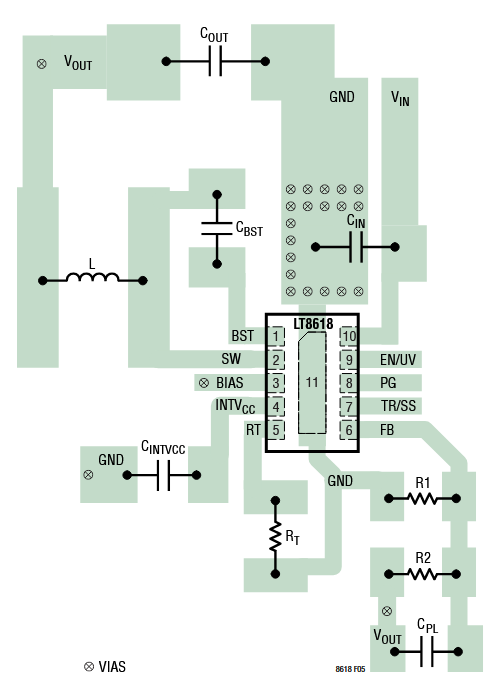
\includegraphics[width=\textwidth]{pcb_layout_LT8618.png}
        %\caption{recommended \gls{acr:pcb} layout of the LT8618 buck converter \autocite{LT8618DatasheetProduct}}
        \label{fig:pcb_layout_LT8618}
    \end{subfigure}
    \hfill
    \begin{subfigure}[b]{0.45\textwidth}
        \centering
        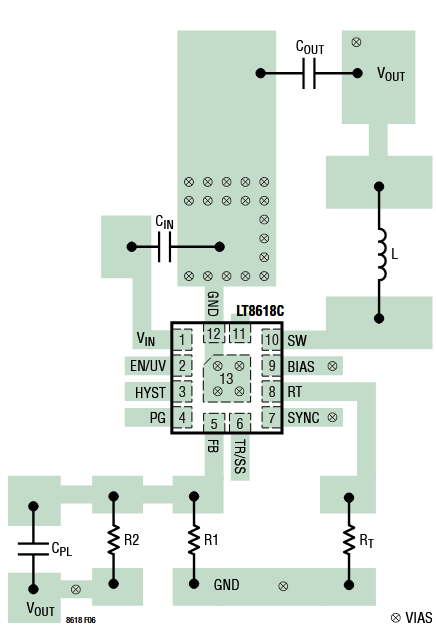
\includegraphics[width=\textwidth]{pcb_layout_LT8618C.png}
        %\caption{recommended \gls{acr:pcb} layout of the LT8618C buck converter \autocite{LT8618DatasheetProduct}}
        \label{fig:pcb_layout_LT8618C}
    \end{subfigure}
    \caption{Recommended PCB layouts for the LT8618 (a) and LT8618C (b) buck converter \autocite{LT8618DatasheetProduct}}
\end{figure}
% EOF